\section{Durchführung}
\label{sec:Durchführung}
\subsection{Technische Daten} \label{sec:Daten}
Im folgenden werden zunächst die technischen Daten der einzelnen Komponenten etc aufgelistet:
\begin{align*}
    \textbf{Dopplerphantomflussigkeit:} && \rho &= 1,15  \unit\gram / \unit{\cubic\centi\meter} & \text{Dichte} \\
    && c_L &= 1800 \unit\meter / \unit\second & \text{Schallgeschwindigkeit} \\
    && \nu &= 12 \unit{\milli\pascal\second} & \text{Viskosität} \\
    \\
    \textbf{Dopplerprisma:} && c_P &= 2700 \unit\meter / \unit\second & \text{Schallgeschwindigkeit} \\
    && l &= 30,7 \unit{\milli\meter} & \text{Länge der Vorlaufstrecke} \\
    \\
    \textbf{Strömungsrohre:} && \text{Innendurchmesser} && \text{Außendurchmesser} \\
    && 7 \unit{\milli\meter} && 10 \unit{\milli\meter} \\
    && 10 \unit{\milli\meter} && 15 \unit{\milli\meter} \\
    && 16 \unit{\milli\meter} && 20 \unit{\milli\meter} \\
\end{align*}

\subsection{Vorbereitungsaufgabe}
Die Dopplerwinkel berechnen sich nach der Formel
\begin{equation}
    \alpha = 90° - \text{arcsin}\left(\text{sin} \theta \frac{c_L}{c_P}\right).
\end{equation}
Daraus folgt für
\begin{align*}
    \theta_1 &= 15° &\implies&& \alpha_1 &= 80,06°, \\
    \theta_2 &= 30° &\implies&& \alpha_2 &= 70,53°, \\
    \theta_3 &= 60° &\implies&& \alpha_3 &= 54,74°. \\
\end{align*}
\subsection{Aufbau}
Der Aufbau besteht aus einem Flüssigkeitskreislauf, an dem eine Zentrifugalpumpe angeschlossen ist.
Die Pumpe erzeugt die Strömung innerhalb der Strömungsrohre. Die Geschwindigkeit des Durchflusses kann stufenlos
durch die Pumpleistung geregelt werden. Innerhalb der Rohre befindet sich die Dopplerphantomflussigkeit.
\begin{wrapfigure}{r}{0.3\linewidth}
    \center
    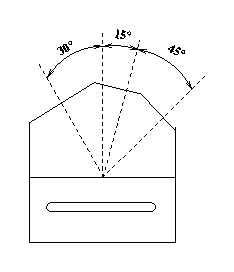
\includegraphics[width=\linewidth]{pictures/Skizze2.pdf}
    \caption{Dopplerprisma.}
    \label{fig:Skizze2}
\end{wrapfigure}
In diesem Kreislauf sind verschiedene Rohrstücke mit verschiedenen Durchmessern eingebaut, siehe dafür \hyperref[sec:Daten]{Kapitel \ref{sec:Daten}}.
Auf diese Rohrstücke wird jeweils ein Dopplerprisma aus Acryl montiert.
Wie in der \hyperref[fig:Skizze2]{Abbildung \ref{fig:Skizze2}} zu erkennen, lassen sich darauf drei Winkel einstellen.
Die Kontaktflächen werden vorher mit einem speziellen Gel bedeckt.
Dass dient der besseren Übertragung der Ultraschallwellen.
Es wird eine Schallfrequenz $\nu_0$ eingestellt.
Die Messsode ist mit dem Computer verbunden. Dort lässt sich direkt über das Programm \enquote{FlowView} die Messwerte ablesen.
\subsection{Durchführung}
